\subsection{Task 3: HVFHV sharing and reporting consistency}
Only Uber (HV0003) and Lyft (HV0005) are used. Pickup time assigns month; a completed trip requires valid pickup/dropoff timestamps and a positive timestamp duration. For each service-month and pickup zone, $V=n_{NN}+n_{YN}+n_{YY}+n_{NY}$. We calculate pooling request rate $(n_{YN}+n_{YY})/V$, reported matched rate $(n_{NY}+n_{YY})/V$, and matching success among requests $n_{YY}/(n_{YN}+n_{YY})$. Missing/other flags are separate from $V$; a zero denominator is undefined. The $N/Y$ category remains in $V$ because it is a required reporting-consistency category.
\begin{table}[htbp]\centering\small\caption{HVFHV sharing rates; denominators are valid-status trips $V$ and pooling requests $Q$.}\label{tab:t3rates}\begin{tabular}{llrrrrr}\hline Month & Service & $V$ & $Q$ & Request \% & Matched \% & Success \% \\ \hline
2026-04 & Uber & 15,378,858 & 417,403 & 2.71 & 1.66 & 61.18 \\
2026-04 & Lyft & 5,617,095 & 1,938 & 0.03 & 0.02 & 3.77 \\
2026-05 & Uber & 15,354,816 & 388,750 & 2.53 & 1.44 & 56.82 \\
2026-05 & Lyft & 6,770,928 & 2,022 & 0.03 & 0.02 & 3.36 \\
\hline\end{tabular}\end{table}
The twelve PNG maps cover all three rates by service and month. For zone comparisons, pooling request and reported matched rates need at least 100 valid-status trips; matching success needs at least 100 requests. Below-threshold zones are marked insufficient sample in gray, not shown as zero. The CSV gives every numerator, denominator, missing/other count, and status. Zones 264/265 remain in the tables but have no drawable polygon.
\begin{figure}[htbp]\centering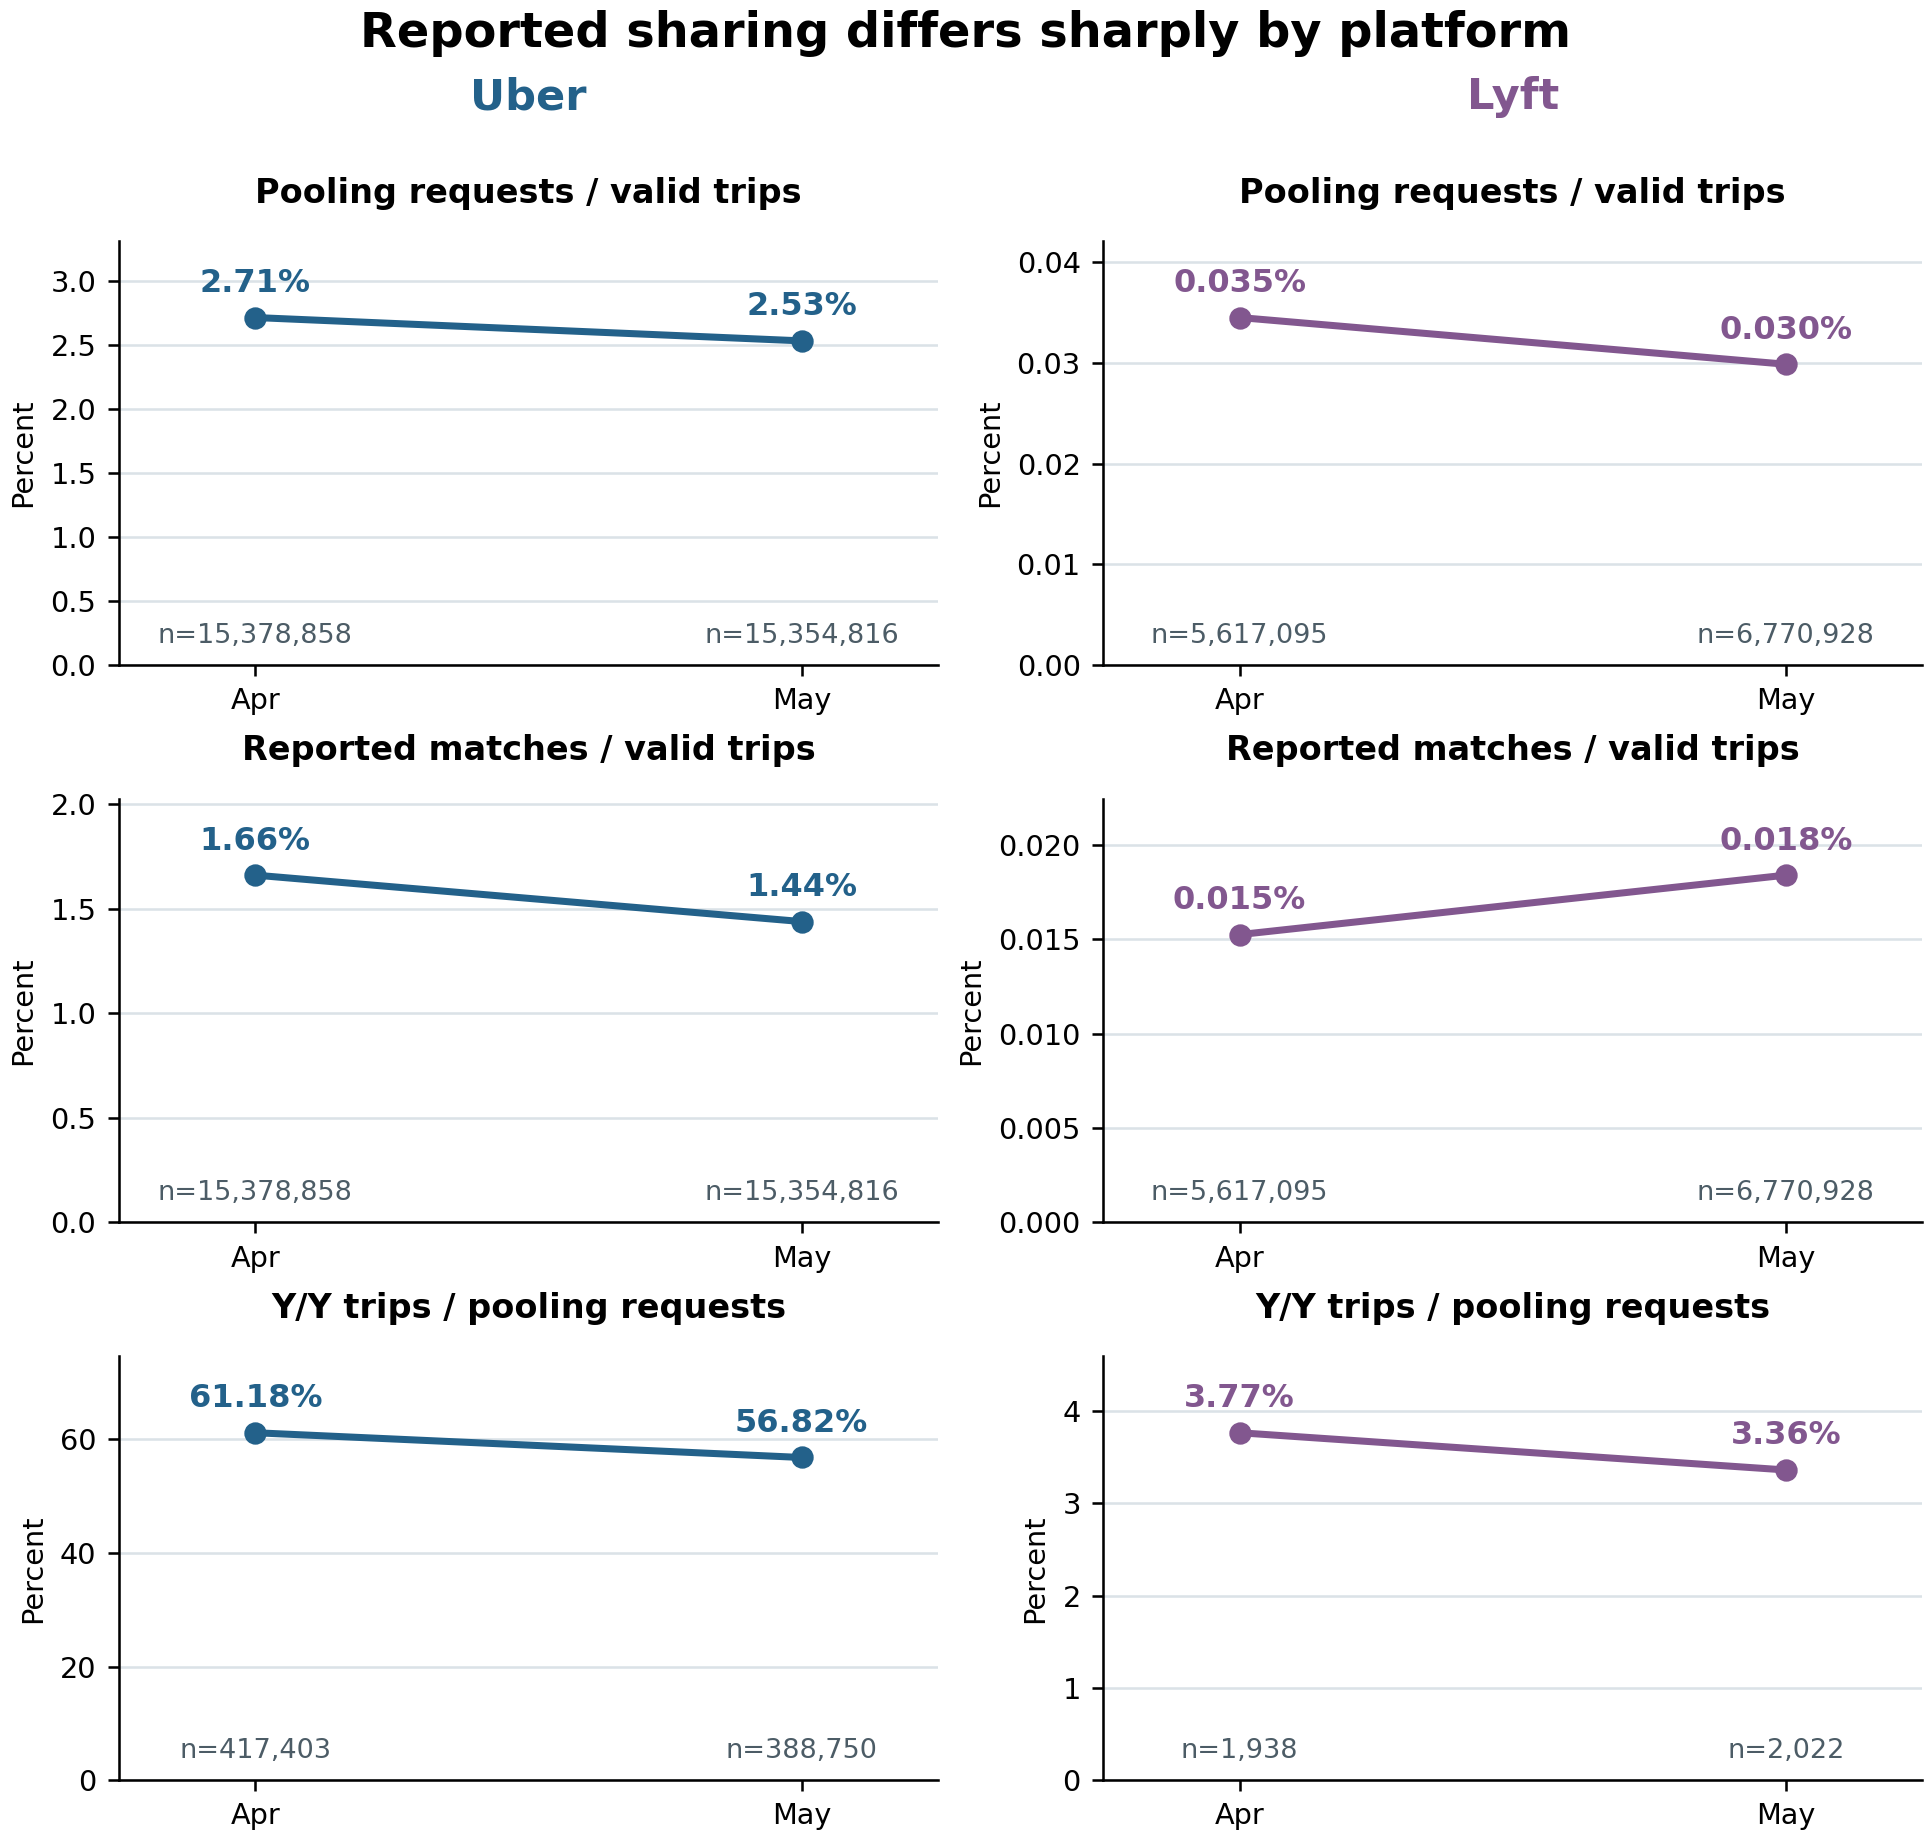
\includegraphics[width=.9\textwidth]{04_Results/Task_3/figures/monthly_sharing_rates.png}\caption{Monthly platform sharing rates. The three panels use their stated denominators.}\label{fig:t3overview}\end{figure}
\begin{figure}[htbp]\centering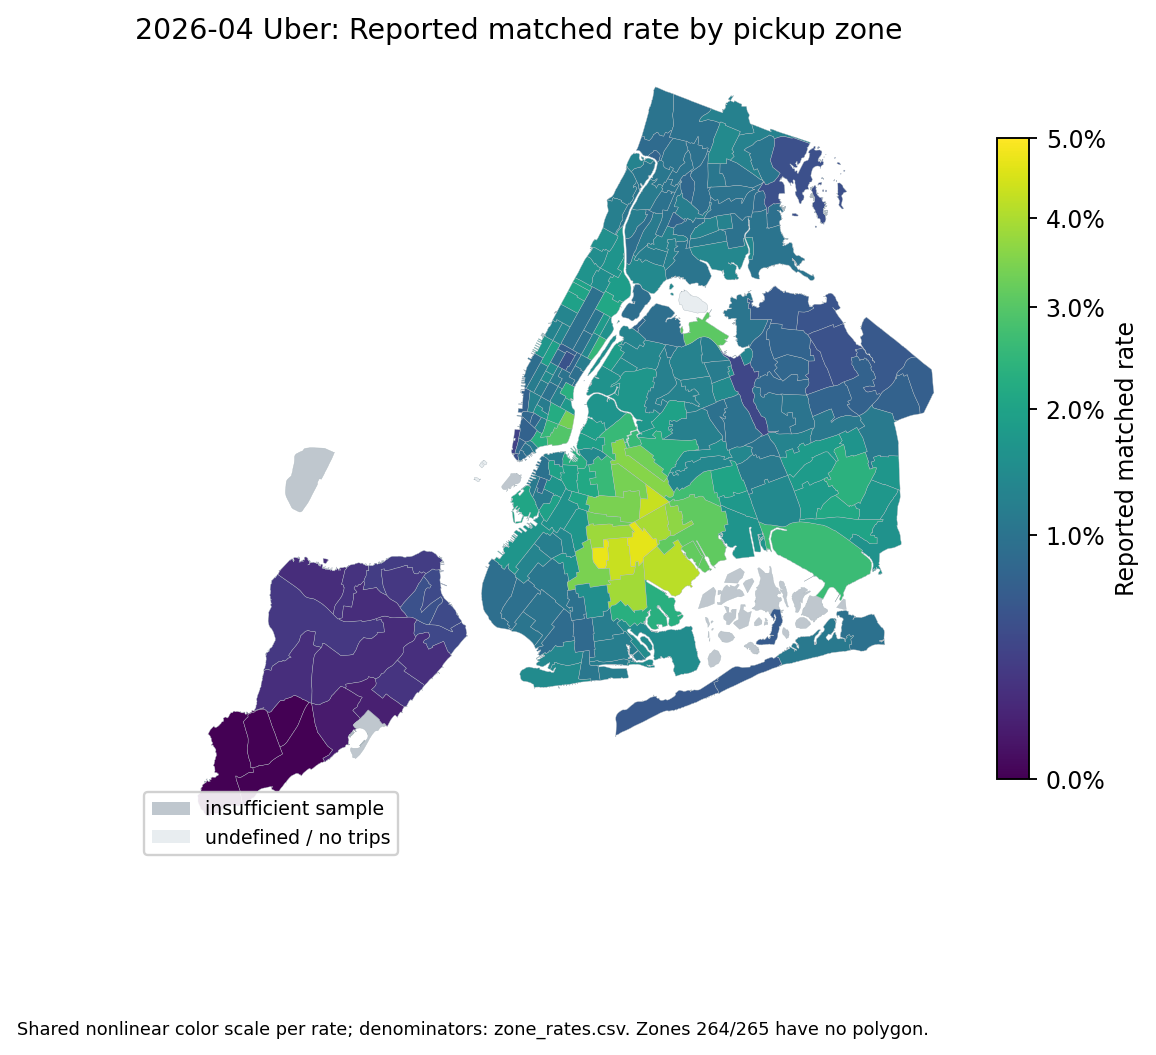
\includegraphics[width=.46\textwidth]{04_Results/Task_3/figures/reported_matched_rate_2026-04_uber.png}\hfill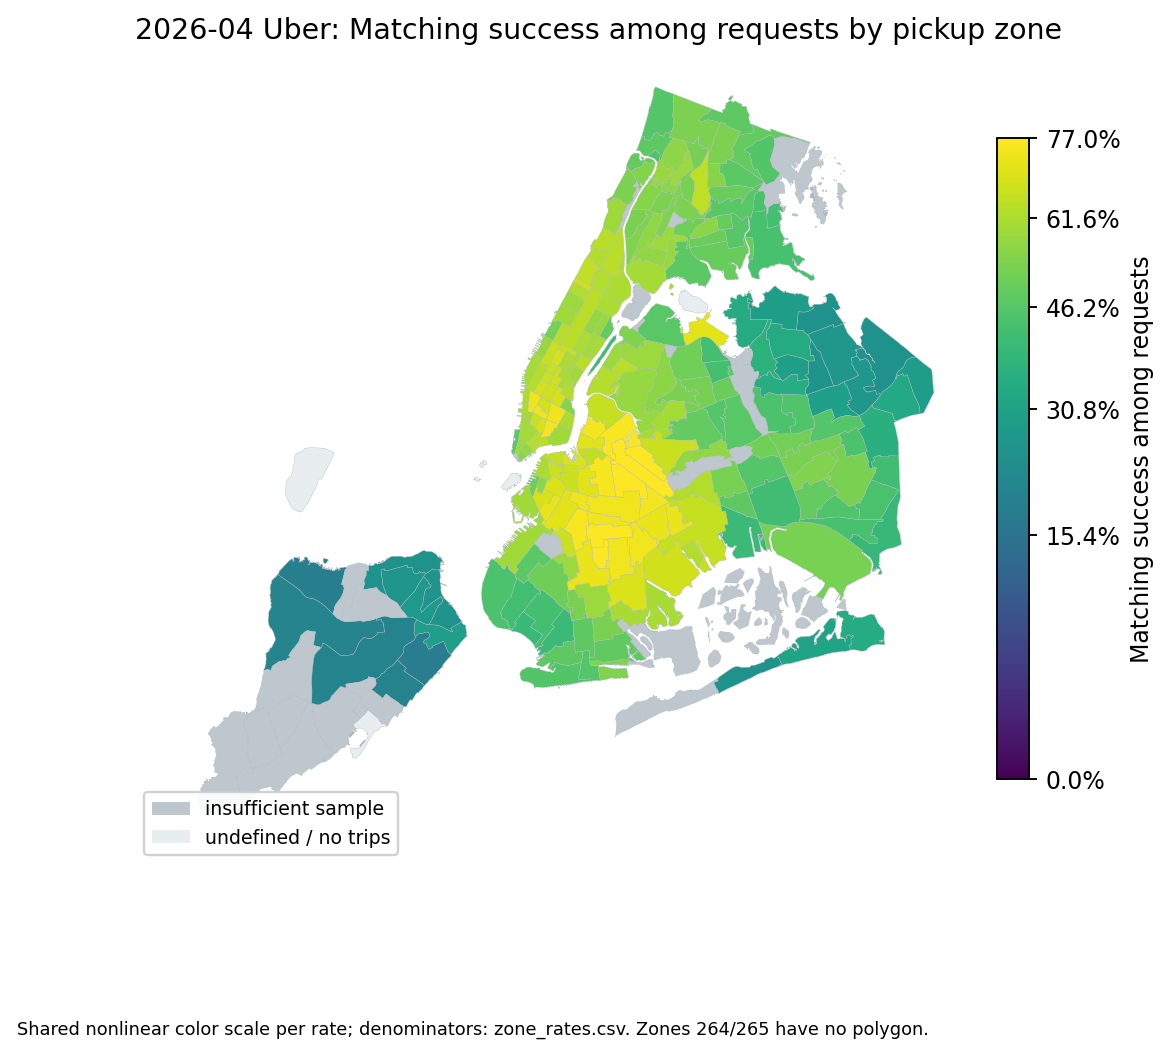
\includegraphics[width=.46\textwidth]{04_Results/Task_3/figures/matching_success_2026-04_uber.png}\caption{April Uber reported matched rate and matching success by pickup zone, with sample thresholds.}\label{fig:t3maps}\end{figure}
In 2026-04, Uber's pooling request rate was 2.71\% and reported matched rate 1.66\%, versus Lyft's 0.03\% and 0.02\%. Uber's matching success among 417,403 requests was 61.18\%; Lyft's among 1,938 requests was 3.77\%.
In 2026-05, Uber's pooling request rate was 2.53\% and reported matched rate 1.44\%, versus Lyft's 0.03\% and 0.02\%. Uber's matching success among 388,750 requests was 56.82\%; Lyft's among 2,022 requests was 3.36\%.
For Uber in 2026-04, 232 pickup zones meet the 100-request matching-success threshold. The highest reported matching success among these is Stuyvesant Heights (76.9\% of 5,173 requests).
For Lyft in 2026-04, 3 pickup zones meet the 100-request matching-success threshold. The highest reported matching success among these is East Chelsea (5.8\% of 241 requests).
For Uber in 2026-05, 233 pickup zones meet the 100-request matching-success threshold. The highest reported matching success among these is Lower East Side (76.0\% of 4,618 requests).
For Lyft in 2026-05, 2 pickup zones meet the 100-request matching-success threshold. The highest reported matching success among these is Midtown South (5.7\% of 175 requests).
No Uber or Lyft records in either month had missing/other request-match statuses after the completed-trip filter. Lyft has $N/Y$ records (783 in April, 1,177 in May); Uber has none. These are counted in reported matches but are not pooling requests.
These are rates among observed completed trips, not among every app request. A reported match does not verify partner identity, overlap duration, or whether the full ride was pooled; $N/Y$ records indicate a flag inconsistency and may inflate the reported matched rate, particularly for Lyft. Differences between services can reflect customer, geography, and product mix rather than platform performance alone.
